\documentclass[12pt]{report}
\usepackage[a4paper]{geometry}
\usepackage[myheadings]{fullpage}
\usepackage{fancyhdr}
\usepackage{lastpage}
\usepackage{graphicx, wrapfig, subcaption, setspace, booktabs}
\usepackage[T1]{fontenc}
\usepackage[font=small, labelfont=bf]{caption}
\usepackage{fourier}
\usepackage[protrusion=true, expansion=true]{microtype}
\usepackage[english]{babel}
\usepackage{sectsty}
\usepackage{url, lipsum}
\usepackage{listings}
\usepackage{float}
\usepackage{todonotes}
\usepackage{stmaryrd}
\usepackage{amsfonts}
\usepackage{amsmath}
\usepackage{bm}
\graphicspath{{images/}}

\lstset{
	basicstyle=\ttfamily,
	columns=fullflexible,
	frame=single,
	breaklines=true,
	postbreak=\mbox{\textcolor{red}{$\hookrightarrow$}\space},
}

\usepackage{hyperref}
\hypersetup{
	colorlinks,
	citecolor=black,
	filecolor=black,
	linkcolor=black,
	urlcolor=black
}

\newcommand{\HRule}[1]{\rule{\linewidth}{#1}}
\onehalfspacing
\setcounter{tocdepth}{5}
\setcounter{secnumdepth}{5}

%-------------------------------------------------------------------------------
% HEADER & FOOTER
%-------------------------------------------------------------------------------
\pagestyle{fancy}
\fancyhf{}
\setlength\headheight{15pt}
\fancyfoot[R]{Page \thepage\ of \pageref{LastPage}}
%-------------------------------------------------------------------------------
% TITLE PAGE
%-------------------------------------------------------------------------------

\begin{document}
	
	\title{ \normalsize \textsc{Large-Scale Data Analysis Techniques}
		\\ [2.0cm]
		\HRule{0.5pt} \\
		\LARGE \textbf{\uppercase{A Review on Multi-Label Learning Algorithms}}
		\HRule{2pt} \\ [0.5cm]
		\normalsize \today \vspace*{5\baselineskip}}
	
	\date{}
	\author{
		Nikiforos Pittaras, M1422\\
		Chrysoula Themeli, M1423 \\ 
		National and Kapodistrian University of Athens\\
		Department of Informatics and Telecommunications }
	
	\maketitle
	\tableofcontents
	\listoffigures
	\newpage
	
	%-------------------------------------------------------------------------------
	% Section title formatting
	\sectionfont{\scshape}
	%-------------------------------------------------------------------------------
	
	%-------------------------------------------------------------------------------
	% Summary of the paper
	%-------------------------------------------------------------------------------
	
	\section*{Introduction}
	\addcontentsline{toc}{section}{Introduction}
	
	\subsection*{Multi-label learning}
	\addcontentsline{toc}{subsection}{Multi-label learning}
	The paper ``A Review on Multi-Label Learning Algorithms'' by Zhang et al.
  studies multi-label learning, applied in supervised classification. Supervised
  classification trains a model $f: X \rightarrow Y$ and for each pair
  $f(x_i,y_i)$, it outputs a real number $r$ that represents the confidence that
  the label $y_i$ characterizes $x_i$. Given $r$ and a thresholding scheme, labels
  are marked as relevant or not relevant to the input data vector $x_i$ (e.g.
  for $r$ representing probability estimates, $r \in [0,1]$, a simple
  thresholding function is $t(x_i) = 0.5$. In other words, labels with outputs
  greater than $0.5$ are assigned to $x_i$ by the model). Standard, single-label learning maps an
  example to a single label, completely ignoring multiple semantics that
  real-objects usually have. On the other hand, multi-label learning allows an
  example/instance $x_i$ to be mapped to more than one label, i.e. to any label
  vector which is a member of the powerset of the label set $Y$. This however
  results to an exponentially growing search space,
  since the size of the latter is an exponential function of the number of labels, i.e. $|\mathbb{P(Y)}| = 2^{|Y|}$.
	
	One straightforward solution is to exploit label correlations. Real objects
  are usually characterized by similar and correlated concepts. For example, if an article is
  characterized by label "football" it follows that it will be also
  characterized by the term "sports" and it is likely that it will be labeled
  with ``crowd'' or ``entertainment''. On the other hand, the label "science"
  will be likely to be irrelevant. Exploiting this label interdependence gives
  rise to techniques that perform better and more efficiently that brute force
  search on the large space of all label sets. The authors categorize approaches
  to three general strategies, according to the extent of label correlation exploitation:
	
	\begin{itemize}
		\item \textbf{First-order strategies: }These algorithms ignore label
      correlations and perform a "one-vs-all" strategy. They often transform a
      multi-label problem into multiple single-label problems, combining the
      result in an aggregation-like manner. Algorithms of this category are
      simple, scalable, have the capability of parallel implementation, but
      offer suboptimal performance.
		\item \textbf{Second-order strategies: }Algorithms in this category consider
      \emph{pairwise} label correlations, i.e. tuples of labels. Having a good
      trade-off between generalization performance and scalability, they
      generally outperform first-order strategies but their limited exploration
      of the label dependency space leads to lacking performance in some real
      world applications.
		\item \textbf{High-order strategies: }These algorithms capture a high degree
      of label correlations, having a large comlexity and strong modeling
      capabilities. This of course leads to increased performance but renders them computationally demanding and less scalable.
	\end{itemize}
	
	\subsection*{Evaluation metrics}
	\addcontentsline{toc}{subsection}{Evaluation metrics}

	With respect to performance evaluation, traditional single-label evaluation metrics are extended to
  incorporate the multi-labeled output. This extension is categorizable into two
  groups. One with respect to the expansion ``axis'' (expansion to multiple examples or labels)
  and the task type (classification or ranking).

    Before proceeding with the metrics, we define the concepts of true positive(TP), false positive(FP),
    true negative (TN) and false negative (FN) of a label $y_j$:
		\begin{itemize}
			\item True positive:  $TP_j = |\{x_i | y_j \in Y_i \wedge y_j \in h(x_i), 1 \leq i \leq p \}|$
			\item False positive: $FP_j = |\{x_i | y_j \notin Y_i \wedge y_j \in h(x_i), 1 \leq i \leq p \}|$
			\item True negative: $TN_j = |\{x_i | y_j \notin Y_i \wedge y_j \notin h(x_i), 1 \leq i \leq p \}|$
			\item False negative: $FN_j = |\{x_i | y_j \in Y_i \wedge y_j \notin h(x_i), 1 \leq i \leq p \}|$
		\end{itemize}

    Many metrics are defined in terms of the above concepts. We proceed to
    present multi-label evaluation metrics.

	\begin{itemize}
		\item \textbf{Example-based: } This type of metrics evaluate multi-labeled
      performance on each example and then the result is spread to the whole
      dataset. The metrics with respect to classification-based and ranking
      based approaches are:
      
		\begin{itemize}
			\item Classification-wise metrics:
			\begin{itemize}
				\item Precision: $P(h) = \frac{1}{p} \sum_{i=1}^{p} \frac{|Y_i \cap h(x_i)|}{|h(x_i)|}$

          Precision measures the proportion of examples correctly classified to $y_i$, out
          of the total examples assigned to the class by the model.
				\item Recall: $R(h) = \frac{1}{p} \sum_{i=1}^{p} \frac{|Y_i \cap h(x_i)|}{|Y_i|}$

          Recall measures the proportion of examples correctly classified to $y_i$, out
          of the total examples assigned to the class in the ground truth.
        \item Subset Accuracy:  $SA(h) = \frac{1}{p} \sum_{i=1}^p \llbracket h(x_i) = Y_i \rrbracket$

          Subset accuracy compares the predicted and ground truth sets for equality.
				\item Hamming Loss: $H(h) = \frac{1}{p} \sum_{i=1}^{p} [h(x_i)\Delta Y_i] $

          The Hamming loss compares the predicted and ground truth sets,
          measuring the set difference of the two.
				\item Accuracy: $A(h) = \frac{1}{p} \sum_{i=1}^{p} \frac{|Y_i \cap h(x_i)|}{|Y_i \cup h(x_i)|}$
          
          Accuracy measures the proportion of examples correctly classified to
          $y_i$, out of the total examples assigned to that class either by the
          model or by the ground truth.
				\item $F^ \beta$ -metric:  $F^ \beta _{exam} (h) = \frac{(1+ \beta ^2) \cdot Precision_{exam}(h) \cdot Recall_{exam}(h)}{\beta ^2 \cdot Precision_{exam}(h) + Recall_{exam}(h)}$
          
          The F-measure combines the precision and recall metrics via a $beta$-
          parameterized harmonic mean.
			\end{itemize}
			\item Ranking-wise metrics:
			\begin{itemize}
				\item One-error: $one-error(f) = \frac{1}{p} \llbracket [argmax_{y \in Y}f(x_i,y)] \notin Y_i \rrbracket$

          The One-error measure checks whether the top ranked class is within
          the ground truth label set.
				\item Coverage:  $coverage(f) = \frac{1}{p} \sum_{i=1}^{p} max_{y \in Y_i} rank_f(x_i,y) - 1$

          The coverage measure counts the steps required to meet all members of
          the ground truh label set in the ranked list, starting from the top.
				\item Ranking loss: $rloss(f) = \frac{1}{p} \sum_{i=1}^{p} \frac{1}{|Y_i| {\overset{\sim}{|Y_i|}}} |\{(y', y'') | f(x_i,y') \leq f(x_i,y''), (y', y'') \in Y_i \times {\overset{\sim}{|Y_i|}} \}| $ 

          The ranking loss measure examines the frequency of reversely ranked
          label pairs.
				\item Average Precision:  $agvprec(f) = \frac{1}{p} \sum_{i=1}^{p} \frac{1}{|Y_i|} \sum_{y \in Y_i} \frac{|\{y' | rank_f(x_i,y') \leq rank_f(x_i,y), y' \in Y_i\}|}{rank_f(x_i,y)}$

          The average precision measures the average of labels in the ground
          truth which are placed higher than $y_i$.
			\end{itemize}
		\end{itemize}
  \item \textbf{Label-based: }
		The label-based metrics are also separated in two perspectives:
		\begin{itemize}
			\item Classification: Let $B(TP_j, FP_j, TN_J, FN_J)$ represent some
        specific binary classification metric $(B \in \{Accuracy, Precision,
        Recall, F^ \beta \})$. The metrics from a classification perspective are the following:
			\begin{itemize}
				\item Macro-averaging: $B_{macro}(h) = \frac{1}{q} \sum_{1}^{q} B(TP_j, FP_j, TN_J, FN_J)$

          Macro-averaging produces the average across all classes.
				\item Micro-averaging: $B_{micro}(h) = B(\sum_{1}^{q}TP_j, \sum_{1}^{q}FP_j, \sum_{1}^{q}TN_j, \sum_{1}^{q}FN_j)$

          Micro-averaging produces class-wise metrics by considering True /
          False Positive / Negative elements from all classes.
			\end{itemize}
			\item Ranking:
			\begin{itemize}
				\item Macro AUC: $AUC_{macro} = \frac{1}{q} \sum_{1}^{q} \frac{|\{(x', x'') | f(x',Y_j) \geq f(x'',Y_j), (x',x'') \in Z_j \times \overset{\sim}{|Z_j|} \}|}{|Z_j|{\overset{\sim}{|Z_j|}}}$
				\item Micro AUC: $AUC_{micro} = \frac{|\{(x',x'',y',y'') | f(x',y') \geq f(x'',y''), (x',y') \in S^+, (x'',y'') \in S^- \}|}{|S^+||S^-|}$

          The AUC (Area Under Curve) evaluation measures the model performance with respect
          to the True and False positive rates. The expansion to the multi-label
          scheme is accomplished by the micro and macro averaging techniques, in
          the same way as above.
			\end{itemize}
		\end{itemize} 
	\end{itemize}
	
	\section*{Multi-label learning algorithms}
	\addcontentsline{toc}{section}{Multi-label learning algorithms}
	In this paper, eight representative multi-label algorithms are presented and analyzed, selected with respect to below criteria:
	\begin{itemize}
		\item[$\checkmark$] Broad, noteworthy and/or unique characteristics
		\item[$\checkmark$] Primitive impact (i.e. leads to a number follow-up related methods)
		\item[$\checkmark$] Favorable influence (popular and/or highly-cited) 
	\end{itemize}
	
	The algorithms to be presented are grouped in two categories:
	\begin{itemize}
		\item \textbf{Problem Transformation Methods: }Algorithms of this category
      transform the multi-labeled problem into into other well-established
      single-labeled learning scenarios, fusing the results into a multi-label output (``Fit data to algorithm'' philosophy)
		\item \textbf{Algorithm Adaptation Methods: }Here, algorithms adapt popular learning techniques to deal with multi-label data directly ("Fit algorithm to data" philosophy)
	\end{itemize}

	\subsection*{Problem Transformation Methods}
  We move on to present the first category of methods, which transform the
  multi-label problem into a set of single label methods. See figure \ref{figure:ptm} for an overview of the approaches examined.

	\addcontentsline{toc}{subsection}{Problem Transformation Methods}
	\begin{figure}[H]
		\centering
		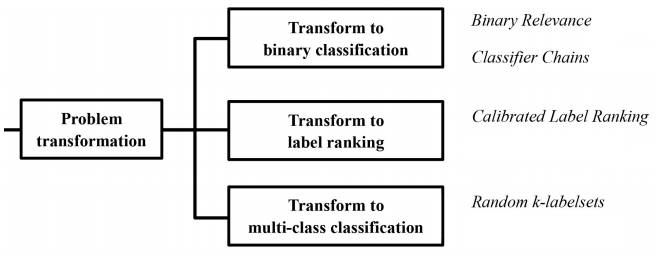
\includegraphics[width=0.9\textwidth]{pt.png}
		\caption{Problem Transformation Algorithms}
		\centering
    \label{figure:ptm}
	\end{figure}

	\subsubsection*{Binary Relevance}
	\addcontentsline{toc}{subsubsection}{Binary Relevance}
	Binary relevance (BR) decomposes the multi-learning problem into $q$
  independent binary classification problems, each of them corresponding to a
  possible label in the label set $Y$. The first task is to construct a
  binary training set for each label, on which a binary learning
  algorithm is used, constructing a classifier that discriminates the
  class $y_j$, i.e. $h_j(\cdot)$. Each training instance is involved in the
  learning process of all $q$ classifiers (cross-training strategy), being 
  regarded as a positive instance in case of relevant labels and negative
  otherwise. For new instances, the algorithm predicts the relevant label set by
  querying each binary classifier and combining the marginal results. A label is
  considered relevant according to the thresholding scheme adopted in the
  multi-label process.
	
	This is a first-order approach algorithm, since it ignores any
  label associations. However, since an one-vs-rest scheme is used and
  classifiers are built and trained for each label separately, the algorithm has the
  advantage of a straightforward parallel implementation. This separation
  however renders the algorithm highly sensitive to class-imbalance in the dataset\footnote{The case where
    the number of positives and negatives for a class differs significantly}.
	
	\subsubsection*{Classifier Chains}
	\addcontentsline{toc}{subsubsection}{Classifier Chains}
	The logic of this algorithm is to transform the multi-label learning problem
  into a chain of binary classification problems, using binary
  classifiers organized in an execution chain. Each classifier is built upon the predictions of
  preceding ones, while the class order is dictated by a permutation function $f_p$. Firstly, a binary training set
  is constructed by enriching each instance with the confidence of preceding
  classifiers, which are iteratively concatenated with the data vector $x_i$.
  The binary algorithm in step $i$ determines whether label $y_i$ is relevant or not for an instance. For
  test instances, the algorithm predicts the relevant labels by iteratively
  traversing the classifier chain producing thresholded confidence scores ($\lambda _{\tau(j)}^x \in {-1, +1}$ in the
  same order as within the training process (i.e., as dictated by $f_p$) represents the predicted binary assignment of $y_{\tau(j)}$).
	
	This is a high-order method that exploits label correlations to a degree, but
  in a random manner.
  It is highly sensitive to the permutation function, since the classifiers'
  ordering directly affects the result. One other disadvantage is that its
  iterative operation prevents parallel implementation, since each classifier 
  has to wait for the results of all previous classifiers in the chain.
  Ensemble schemes can be used to search for and select favorable permutation functions $f_p$.
	
	\subsubsection*{Calibrated Label Ranking}
	\addcontentsline{toc}{subsubsection}{Claibrated Label Ranking}
	This algorithm transforms the learning problem into a pairwise label
  comparison ranking problem. For $q$ labels, $q(q-1)/2$ binary classifiers are
  constructed to discriminate between each label pair via a binary
  classification algorithm $h_{jk}(x)$. Firstly, respective pairwise training
  sets $D_{jk}$ are constructed, where $D_{jk}: \{x_i, Y_i | y_j \in Y_i \oplus
  y_k \in Y_i\}$, i.e. each $D_{jk}$ contains examples either in class $j$ or
  $k$. The learning system votes for each example and if $h_{jk}(x)>0$, then
  $x_i$ is associated with label $y_j$, otherwise $y_j$ is irrelevant and $x_i$
  is assigned to $y_k$. For unknown instances, all classifiers' votes are
  aggregated and ranked. In addition, a virtual label $y_v$ is used as an
  artificial splitting point between relevant and irrelevant labels, serving as
  a decision threshold for label relevance.
	
	This is a second-order approach algorithm using a one-vs-one scheme. The
  advantage of this method is that it smooths out the class-imbalance problem
   by operating on label pairs. The disadvantage is that the number of
  classifiers is quadratic to $|Y|$, compared to the linear complexity for Binary Relevance or
  Classifier Chains algorithms. However, the performance can be improved by
  using pruning methods to reduce the labelset search space.
	
	\subsubsection*{Random k-Label Sets}
	\addcontentsline{toc}{subsubsection}{Random k-Label Sets}
	The random k-label sets algorithm transforms the multi-label learning problem
  into an ensemble of multi-class classification problems. Each such partition
  targets a random subset of $\mathbb{P}(Y)$, limited to subsets present in the
  training dataset $X$, classifying it using Label Powerset (LP) techniques.
  These techniques involve transforming the multi-label dataset into
  single-label data by treating each distinct label set as a new class. Thus, each training example
  is mapped to a new, single class and classified through some single-label multiclass
  classification method. An instance $x_i$ is assigned to a label $y_i$ when the
  votes received for $y_i$ from the ensemble exceed half the max possible that
  this label can get.
  For unseen instances $x_j$, LP predicts its associated label set $Y_j$ by
  querying the single-label predictions of the LP multi-class classifiers and then mapping these
  results it back to the labelsets in $\mathbb{P}(Y)$.
	
	This is a high-order approach algorithm since it utilizes a variety of label correlations. However, there are two limitations in terms of practical feasibility: 
	\begin{itemize}
		\item[$\diamond$] \emph{Incompleteness: }The algorithm is data-sensitive and cannot generalize to label sets that do not appear into the training set.
		\item[$\diamond$] \emph{Inefficiency: }A large label set $Y$ implies high training complexity and extremely few training examples for some newly mapped classes.
	\end{itemize}

	A simple but powerful modification is the Random k-Label Sets variant, which
  runs an ensemble of executions, each with $k$-sized label sets. The ensemble
  scheme improves on the predictive completeness of the system, while the
  limited label set size guarantees computational efficiency. Additionally,
  pruning distinct label sets which are less frequent than a specified threshold is
  another common strategy to improve the method's performance.
	
	\subsection*{Algorithm Adaptation Methods}
  The next category refers to algorithm adaptation methods, i.e. strategies that
  directly address the multi-label nature of the problem. See figure
  \ref{figure:aam} for an overview of the approaches examined.

	\addcontentsline{toc}{subsection}{Algorithm Adaptation Methods}
	
	\begin{figure}[H]
		\centering
		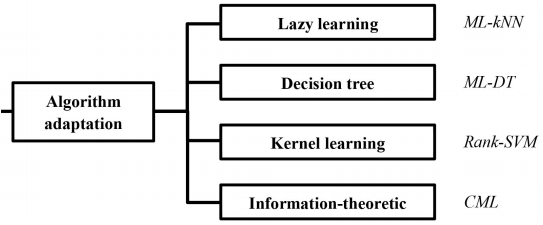
\includegraphics[width=0.9\textwidth]{aa.png}
		\caption{Algorithm Adaptation Methods}
		\centering
    \label{figure:aam}
	\end{figure}

	\subsubsection*{Multi-Label k-Nearest Neighbor (ML-kNN)}
	\addcontentsline{toc}{subsubsection}{Multi-Label k-Nearest Neighbor (ML-kNN)}
	The ML-kNN algorithm adapts nearest neighbor techniques to the multi-label
  setting by utilizing the maximum a posteriori (MAP) rule. The method produces
  predictions by taking into account the labeling information embodied in the neighbors. For new
  instances $x$, the set $N(x)$ represents its $k$ nearest neighbors
  identified in the dataset by a specified similarity or distance measure. Let
  $H_j \equiv (y_j \in Y_i)$, $C_j = \sum_{x_k \in N(x_i)} [\delta(y_j \in
  Y_k)]$, i.e. $H_j$ is the event that $\textbf{x}$ has the label $y_j$ and
  $C_j$ records the number of neighbours of $x$ that have the label $y_j$. Moreover,
  $P(H_j|C_j)$ is the posterior probability that $H_j$ holds in the condition
  that $\textbf{x}$ has exactly $C_j$ neighbors. The posteriors $P(H_j|C_j)$ are
  calculated using Bayes' theorem with respect to the priors and the likelihoods.

	The prior probabilities ($P(H_j)$, $P(\neg H_j)$) are computed via a frequency
  counting strategy, where a smoothing parameter $s$ is used to control the
  effect of uniform prior on the estimation (a common value is  $s=1$). In addition, likelihoods $P(C_j|H_j)$ and $P(C_j| \neg H_j)$ are computed using two frequency arrays:
	\begin{itemize}
		\item $\kappa(r)$, the number of examples labelled $y_j$ with $r$ neighbours labelled $y_j$
		\item $\overset{\sim}{\kappa}(r)$, the number of examples not labelled $y_j$ with $r$ neighbours labelled $y_j$
	\end{itemize}
	 
	This algorithm is a first-order approach that uses Bayesian reasoning. Being a
  nearest-neighbour method, the decision boundary can be modified on-line when
  new instances appear. Moreover, the use of prior probabilities can amend the
  class imbalance issue to a degree. A number of extensions have been proposed that take into account label associations.
	
	\subsubsection*{Multi-Label Decision Tree (ML-DT)}
	\addcontentsline{toc}{subsubsection}{Multi-Label Decision Tree (ML-DT)}
	This method adapts decision tree techniques for multi-label classification.
  Using the multi-label entropy measure, a decision tree is built recursively by
  splitting features in positions such that a maximum information gain is produced. Let $T = \{(x_i,
  Y_i) | 1 \leq i \leq n \}$ be the multi-label dataset with $n$ examples. The
  algorithm splits the $x$ vector at the feature $l$ that maximizes the
  information gain criterion, where $\theta$ is the value in that position. This
  partitions the dataset $T$ into branches ($T^-$ \& $T^+$), where $x_{il} \leq
  \theta, x_i \in T^-$ and $x_{il} > \theta, x_i \in T^+$. This process is
  invoked recursively by treating each new branch as the new
  root node and terminates until some stopping criterion $C$ is met (e.g.
  subtree size). Each label subset is treated as a new class and the single-label entropy is computed. Any new instances are assigned the label of the majority of members of the leaf that they arrive.
	
	In order to ensure low computational cost and high efficiency, the algorithm
  assumes independence among the labels; thus, it is a first-order approach.
  Extensions are proposed to reduce computational cost and exploit label interrelations, such as pruning and ensemble strategies.
	
	\subsubsection*{Ranking Support Vector Machine (Rank-SVM)}
	\addcontentsline{toc}{subsubsection}{Ranking Support Vector Machine (Rank-SVM)}
	Rank-SVM adapts the maximum margin strategy to the multi-label classification
  problem. $q$ linear classifiers are optimized with the empirical
  ranking loss. The learning system is composed by classifiers that distinguish
  between relevant and irrelevant pairs. Each classifier is parameterized with $W = \{w_j,b_j | 1 \leq j \leq q\}$, where $w_j \in \mathbb{R}^d$ and $b_j \in \mathbb{R}$ are the weight vector and the bias
	for the j-th class label $y_j$, respectively. Rank-SVM defines the system’s
  margin on $(x_i,Y_i)$ by considering its ranking ability on the relevant and
  irrelevant label pairs of $x_i$ $(y_j,y_k) \in Y_i \times \bar Y_i$, which are
  separated by a function of their classifiers $h_j, h_k$: $\left<w_j-w_k, x_i
  \right> + b_j - b_k=0$. The margin is defined as the minimum distance from all
  related-unrelated pairs and is minimized along with the training loss
  function. At consistent training, the classifier will return positive margin
  for each training example, since the singed distance will be positive with
  respect to relevant label hyperplanes and negative for irrelevant ones.
  For new test instances, the algorithms retrieves a ranked list of label pairs, ordered
  according to the signed distance to the separation hyperplane.
	
	Non-linear problems can be managed by exploiting kernel feature mapping via
  the kernel trick, which is popular in SVM methods. The optimization method is
  a convex quadratic programming problems and can thus be solved by any QP
  solver.
  This algorithm is a second-order approach as it utilizes pairwise label associations.
  It is adaptable to a variety of tasks and data by using alternative loss
  functions and kernel feature mapping. Kernel selection for the latter can be accomplished by
  multiple kernel learning (MKL) techniques.

  \subsubsection*{Collective Multi-Label Classifier}
	 \addcontentsline{toc}{subsubsection}{Collective Multi-Label Classifier}
   The CML method is a multi-label variant of Conditional Random Field methods.

	 This algorithm involves computing a joint probability distribution on $x, Y$
   where label sets are encoded as binary random vectors and label correlations are encoded into the
   distribution as constraints.
   The conditional $p(\bm{y} | x)$ is computed via the maximum entropy
   criterion, where the information entropy measure $H_p(x,\bm{y})$ is maximized subject to each constraint.
   The latter are modeled as $ \mathbb{E} [ f_k(x,\bm{y}) ] = F_k  $, where $F_k$ is
 learned from the training data.
 The optimal solution is arrived at via Lagrange multipliers, assuming Gaussian
 priors for the variables involved, and has the form of a Gibbs probability
 distribution.
 Test instances are labelled with respect to $\text{argmax}_y\text{ }p(\bm{y} | x)$.


   This is a second-order approach, where all label pairs are considered and not
   just the relevant-irrelevant ones which was the case with the Rank-SVM approach. It is a
   convex constraint optimization problem, and is thus solvable by off the shelf
   CP solvers. The argmax operation during inference is expensive, which renders
   the method very computationally inefficient for large label spaces, if
   pruning is not applied. Finally, varying the expression form of the constraints gives rise to difference
   version of the CML method.
	 
	 \subsection*{Summary of Multi-Label Learning Algorithms}
	 \addcontentsline{toc}{subsection}{Summary of Multi-Label Learning Algorithms}
	 
	 \begin{figure}[H]
	 	\centering
	 	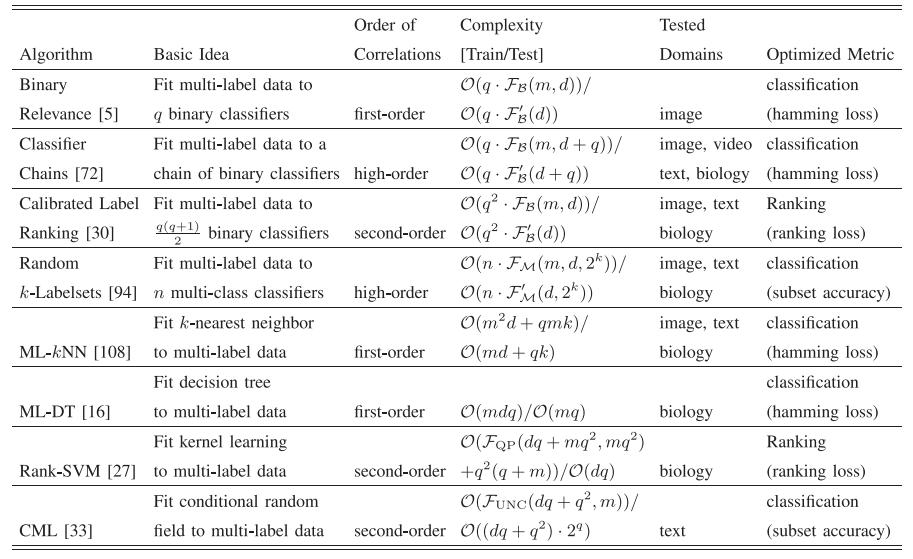
\includegraphics[width=1\textwidth]{summary.png}
	 	\caption{Summary of Multi-Label Learning Algorithms}
	 	\centering
	 \end{figure}
 
 	\section*{Related Learning Methods}
 	\addcontentsline{toc}{section}{Related Learning Methods}
 	Four related learning methods are mentioned in this paper, which are summarized below:
 	\begin{enumerate}
 		\item \textbf{Multi-instance learning: }This method studies the problem
      where each example is described by a bag of instances while associated
      with a single binary label. The bag is assigned a positive label in the
      case of at least one positively labelled member. It models complex
      semantics of $x_i$ in \emph{input space} (i.e. in the variability of each
      bag of instances) rather than its output (i.e. the different labels in the instance's
      label set).
 		\item \textbf{Ordinal classification: } This scheme assumes label relevance
      to an instance is not binary but graded, producing a vector of ordinal graded
      membership of $x$ to a label. Multi-label classification is induced via a
      transformation of the original problem into a set of ordinal problems.
 		\item \textbf{Multi-task learning: }This method studies the problem where
      multiple tasks are trained in parallel. Tasks can share information, and
      knowledge from related tasks is used as an inductive bias to help improve
      the generalization performance of other tasks. The  tasks can share a
      common feature space or use different representations, as is common in
      multi-label learning. In this setting, it is reasonable to have small task
      workloads, since the execution is of a parallel nature. 
 		\item \textbf{Data streams classification: } Here, data is generated in real
      time, corresponding to the real-time nature of some task. Apart from the
      tight temporal constraints, the defining challenge here is the concept
      drift problem, where the concept classified can change over time. A common
      strategy to this effect is to gradually discount the significance of past
      data in favor of newly arrived batches.
     
 	\end{enumerate}
 	
	\section*{Conclusion}
	\addcontentsline{toc}{section}{Conclusion}
	Summarizing, this paper defines the multi-label learning problem, presenting
  an outline of evaluation methods and describing 8 multi-label learning
  representative algorithms. It closes by mentioning some learning scenarios
  related to multi-label learning.

  
  Some important future goals in the field are the formal description of the
  underlying concept behind label correlations, and of the mechanism by which interdependencies ought to
  be handled and modelled in learning problems - especially in large output spaces. 
  In addition, thorough experimental comparative studies are essential to
  discover the advantages and disadvantages of different multi-label learning
  algorithms, so as to aid the conquest of the aforementioned theoretical goal.

  Some online resources on multi-label learning are presented on figure \ref{figure:resources}.
	
	\begin{figure}[H]
		\centering
		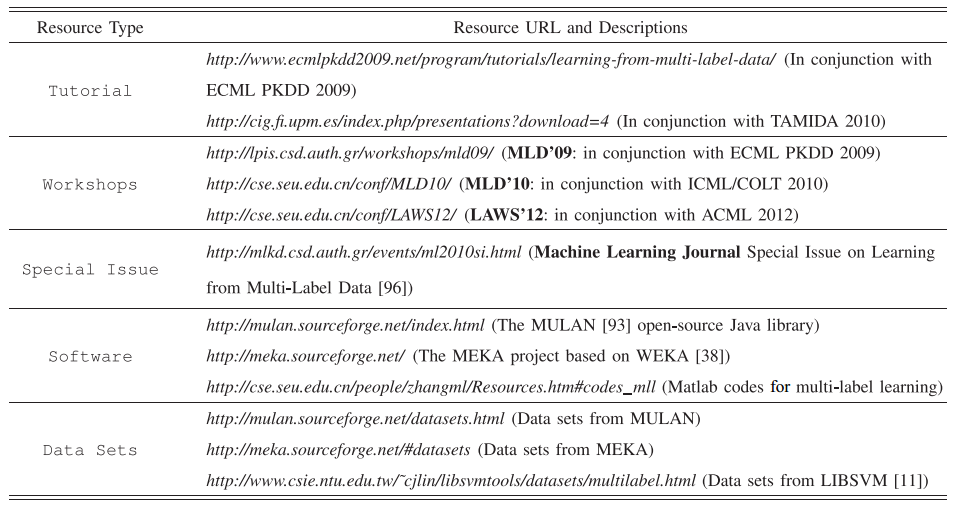
\includegraphics[width=1\textwidth]{online.png}
		\caption{Online resources for Multi-Label Learning}
    \label{figure:resources}
	\end{figure}
	
	%-------------------------------------------------------------------------------
	% REFERENCES
	%-------------------------------------------------------------------------------
	\addcontentsline{toc}{section}{Related Work and Bibliography}
	\renewcommand\bibname{Related Work and Bibliography}
	\begin{thebibliography}{9}
		\bibitem{comp} 
		Madjarov, Gjorgji, et al. "An extensive experimental comparison of methods for multi-label learning." Pattern Recognition 45.9 (2012): 3084-3104
		\bibitem{overview} Tsoumakas, Grigorios, and Ioannis Katakis. "Multi-label classification: An overview." International Journal of Data Warehousing and Mining 3.3 (2006)
		\bibitem{correlations} Zhang, Min-Ling, and Kun Zhang. "Multi-label learning by exploiting label dependency." Proceedings of the 16th ACM SIGKDD international conference on Knowledge discovery and data mining. ACM, 2010


\bibitem{trees} Vens, Celine, et al. "Decision trees for hierarchical multi-label classification." Machine Learning 73.2 (2008): 185-214.
\bibitem{rkl} Tsoumakas, Grigorios, and Ioannis Vlahavas. "Random k-label sets: An ensemble method for multilabel classification." Machine learning: ECML 2007 (2007): 406-417.
\bibitem{mlknn} Zhang, Min-Ling, and Zhi-Hua Zhou. "ML-KNN: A lazy learning approach to multi-label learning." Pattern recognition 40.7 (2007): 2038-2048.
\bibitem{rksvm} Elisseeff, André, and Jason Weston. "A kernel method for multi-labelled classification." Advances in neural information processing systems. 2002.
\bibitem{cml}  Ghamrawi, Nadia, and Andrew McCallum. "Collective multi-label classification." Proceedings of the 14th ACM international conference on Information and knowledge management. ACM, 2005.
\bibitem{ordinals}  Cheng, Weiwei, Eyke Hüllermeier, and Krzysztof J. Dembczynski. "Graded multilabel classification: The ordinal case." Proceedings of the 27th international conference on machine learning (ICML-10). 2010.
      
	\end{thebibliography}
\end{document}
